\documentclass[11pt,a4paper]{article}
\usepackage[english]{babel}
\usepackage[utf8]{inputenc}
\usepackage{amsmath, amssymb}
\usepackage{graphicx}
\usepackage{caption}
\usepackage{float}
\usepackage[top=1in, left=1.25in, right=1.25in, bottom=.8in]{geometry}
\usepackage[numbered,framed]{matlab-prettifier}
\usepackage{filecontents}
\usepackage[T1]{fontenc}
\usepackage{bigfoot}
\usepackage{listings}

\numberwithin{equation}{subsection}
\newcommand{\eqname}[1]{\tag*{#1}}

\begin{filecontents}{h5.m}
%% Load video
close all; clear all; clc;
vid = VideoReader('video/double_pendulum.mp4');
height = vid.Height; width = vid.Width; 
numFrames = round(vid.Duration * vid.FrameRate);
t = linspace(0, vid.Duration, numFrames); dt = t(2)-t(1);
X = zeros(height*width, numFrames);
for ii=1:numFrames
    vidFrame = rgb2gray(readFrame(vid));
%     imshow(vidFrame);
    vec = vidFrame(:); % vectorize video frame
    X(:, ii) = vec;
end

%% Create DMD data matrices
clear vidFrame vid vec ii
X1 = X(:, 1:end-1); X2 = X(:, 2:end);
[U2, Sigma2, V2] = svd(X1, 'econ');
r = 300; % reconstruction rank
U = U2(:, 1:r); Sigma=Sigma2(1:r,1:r); V=V2(:,1:r);
Atilde = U'*X2*V/Sigma;
[W,D] = eig(Atilde);
Phi=X2*V/Sigma*W;
mu=diag(D);
omega=log(mu)/dt;
b = Phi\X1(:, 1); % pseudo-inverse initial conditions
time_dynamics = zeros(r, length(t)); % DMD reconstruction for every time point
for iter = 1:length(t)
    time_dynamics(:, iter) = (b.*exp(omega*(t(iter))));
end
Xdmd = Phi*time_dynamics;   % DMD resconstruction with all modes

%% Background subtraction
clear time_dynamics W D Atilde mu b U Sigma V X1 X2 U2 V2
Xres = reshape(X, height, width, numFrames);
Xlow = reshape(Xdmd, height, width, numFrames);
Xsparse = Xres-abs(Xlow);
R = Xsparse; R(R>0)=0;
Xlow = R+abs(Xlow);
Xsparse = Xsparse-R; % remove negative intensities

%% Plots
clear Xdmd X R
keyFrame = 100;
% Low rank reconstruction by DMD
figure(1), imshow(uint8(Xsparse(:, :, keyFrame)+Xlow(:, :, keyFrame)))
title(strcat('DMD reconstruction (rank ', num2str(r), ')')); set(gca, 'Fontsize', 12)
% Foreground object
figure(2), imshow(12*uint8(Xsparse(:, :, keyFrame)))
title(strcat('Foreground (rank ', num2str(r), ')')); set(gca, 'Fontsize', 12)
% Background object
figure(3), imshow(0.8*uint8(Xlow(:, :, keyFrame)))
title(strcat('Background (rank ', num2str(r), ')')); set(gca, 'Fontsize', 12)
% SVD spectrum
figure(4), plot((diag(Sigma2)/sum(diag(Sigma2)))*100, 'ro-', 'Markersize', 10, 'Linewidth', 1.5)
xlabel('Modes'); ylabel('% of Energy captured');
title(strcat('SVD specturm (rank ', num2str(r), ')'))
ylim([0 100])
set(gca, 'Fontsize', 12)
set(gcf, 'Position',  [200, 100, 800, 600])

%% Visualization
figure(1)
for kk = 1:numFrames
    imshow(15*uint8(Xsparse(:, :, kk)))
end
\end{filecontents}

\let\ph\mlplaceholder % shorter macro
\lstMakeShortInline"
\lstset{
  style              = Matlab-editor,
  basicstyle         = \mlttfamily,
  escapechar         = ",
  mlshowsectionrules = true,
}

\title{Amath 482 Winter 2019 \\
HW5: Background Subtraction in Video Streams}
\author{Wenrui Yuan}
\date{\today}

\begin{document}
\maketitle

\begin{abstract}
	We will be exploring the Dynamical Mode Decomposition (DMD) method in separating foreground and background objects in various video streams. Three videos capturing moving objects with backgrounds will be tested to examine the efficiency of DMD algorithm and low-rank reconstruction of SVD method.
\end{abstract}

\section{Introduction and Overview}
Video background subtraction is a widely used method for moving objects detection. Such technique is very helpful for surveillance tracking and human poses estimation.\cite{fore} In particular, we will be examining the DMD reconstruction on three videos to understand how DMD method performs the background subtraction and its correlation with the rank number as well as the varying performance in different scenarios.\\
Particularly, the first video will be studying relatively simple moving double pendulum on a stationary background. The second one will be a man giving a presentation with more complex movements captured by a stationary camera while the third one will also be studying complex movements with a non-stationary camera. Three tests will be performed to collectively test advantages and limits of the DMD method.
\section{Theoretical Background}
\subsection{Dynamic Mode Decomposition (DMD)}
The Dynamic mode decomposition method (DMD) is a combination of dimensionality reduction algorithms.\cite{dmd1} This method takes spatial snapshot data $"x"_k$ from a dynamical system at some time $t_k$. DMD maps 
these data regressively to a linear dynamical system $"x"_{k+1}="A""x"_k$, where $"A"$ is chosen to minimize $\|"x"_{k+1}-"Ax"_k\|_2$ over the $k=1, 2, \cdots, k-1$ snapshots.\cite{dmd1}\cite{dmd2}. Algorithm applied in this report will be based on SVD for minimizing numerical errors over long term truncation.\\
Since we will be focusing on separating foreground and background, consider the DMD spectrum of frequencies
\begin{equation}
"X"_{\text{DMD}}=\underbrace{b_p\varphi_pe^{\omega_pt}}_\text{Background}+\underbrace{\sum_{j\neq p}b_j\varphi_je^{\omega_jt}}_\text{Foreground}
\end{equation}
where $b_p\varphi_pe^{\omega_pt}$ represents the background with the assumption that $\|\omega_p\|\approx0, p\in\{1, 2, \cdots, \ell\}$ and $\sum_{j\neq p}b_j\varphi_je^{\omega_jt}$ represents the foreground object satisfying that $b_j\varphi_je^{\omega_jt}\in\mathbb{C}^{n\times m}\text{ }\forall\text{ } j$ and $\forall\text{ } j\neq p, \|\omega_j\|$ is bounded away from zero.\\
Thus, we can consider the low-rank reconstruction and sparse reconstruction,
\begin{equation}
"X"_{\text{DMD}}^{\text{Low-Rank}}=b_p\varphi_pe^{\omega_pt}\qquad\qquad "X"_{\text{DMD}}^{\text{Sparse}}=\sum_{j\neq p}b_j\varphi_je^{\omega_jt}
\end{equation}
as $"X"="X"_{\text{DMD}}^{\text{Low-Rank}}+"X"_{\text{DMD}}^{\text{Sparse}}$ should hold. In this case the sparse reconstruction can be calculated with real-valued elements as
\begin{equation}
"X"_{\text{DMD}}^{\text{Sparse}}="X"-|"X"_{\text{DMD}}^{\text{Low-Rank}}|
\end{equation}.
By taking the modulus of the low rank reconstruction, there could be negative values in $"X"_{\text{DMD}}^{\text{Sparse}}$, but we can store these negative residues into a $n\times m$ matrix "R" so that we have
\begin{equation}
"X"_{\text{DMD}}^{\text{Low-Rank}}\leftarrow"R"+|"X"_{\text{DMD}}^{\text{Low-Rank}}|\qquad "X"_{\text{DMD}}^{\text{Sparse}}\leftarrow "X"_{\text{DMD}}^{\text{Sparse}}-"R"
\end{equation}


\section{Algorithm Implementation and Development}
\begin{itemize}
\item[] \textbf{Load video data and store in to a matrix\\}
Initially, we will compute other parameters like number of frames, video height and width and the time interval discretized by the number of frames and change in time "dt". Also, as we only care about the motion, we need to transform the image in each frame into a grayscale one.

\item[] \textbf{Take SVD of the data matrix and perform a low rank truncation\\}
Note that before SVD, we have to have two slightly different spatial temporal patterns "X1" and "X2".

\item[] \textbf{Take projection of \texttt{A} onto POD modes and the eigen decomposition of such projection\\}
The "rxr" projection "Atilde" is more practical in terms of computation, and is obtained by the low rank truncation of "U", "V" and "Sigma". We then take the eigen decomposition of "Atilde" to obtain eigenvalues, which is from the diagonal of "D" and eigenvectors, which is from the columns of "W".

\item[] \textbf{Compute DMD modes\\}
Note that we are, in fact, computing the eigenvectors of "A", given by columns of "Phi".

\item[] \textbf{Compute DMD spectrum and obtain the DMD solution\\}
The DMD spectrum is obtained from "D", then we take the pseudo inverse of initial conditions as well as create a matrix for DMD reconstruction for each time point. This will give us the DMD solution which helps us to perform DMD reconstruction with all modes.

\item[] \textbf{Reshape correlated data matrices and perform Background subtraction}\\
We reshape the reconstructed and original data matrices into a 3 dimensional ones with first two dimension be the height and width of the video. Then compute the sparse reconstruction by subtracting the background from the original matrix. But this will give us negative values. We thus make a matrix "R" to store "Xsparse" and filter out all positive values and keep only negative residues. By finally removing these negative values in the sparse reconstruction, we obtain both foreground and background data.
\item[] \textbf{Plot DMD reconstructed video Foreground videoand Background video, as well as the SVD spectrum}
\end{itemize}


\section{Computational Results}
\begin{figure}[H]
\begin{center}
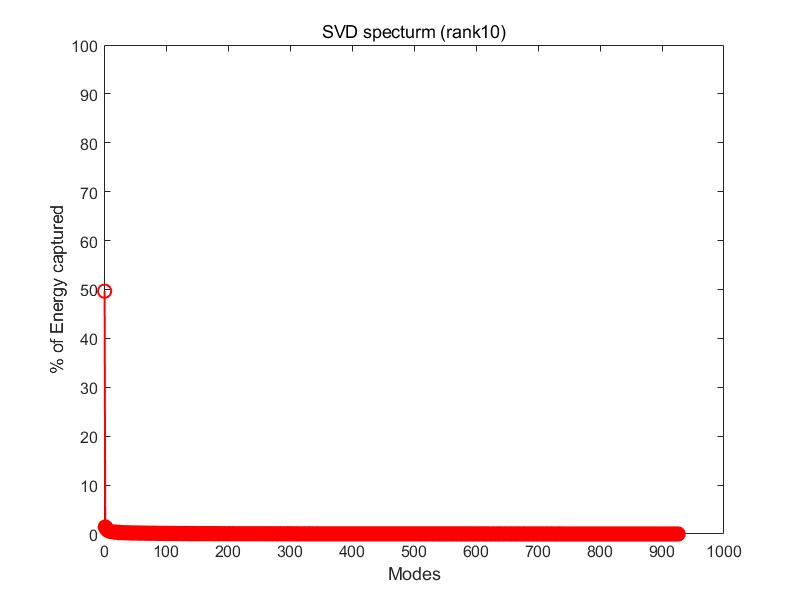
\includegraphics[scale=0.25]{t1f0.jpg}
\caption{SVD spectrum of energy captured by each mode (Test 1)}
\end{center}
\end{figure}
As we can see in figure 1, the motion of double pendulum is relatively simple, energy captured by first few modes are very high so that we can have a good approximation with very low rank

\begin{figure}[H]
\begin{center}
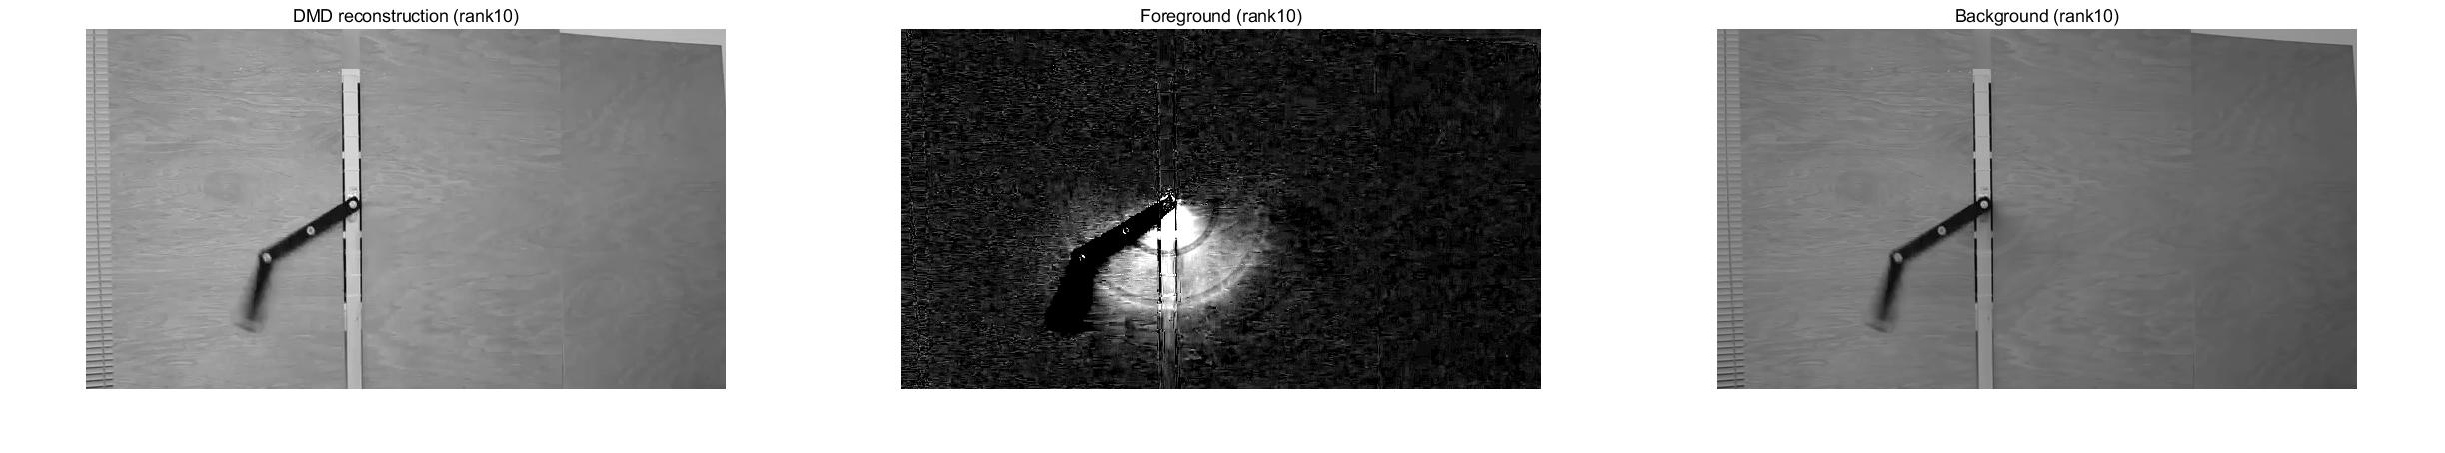
\includegraphics[scale=0.17]{t1f1.jpg}
\caption{DMD reconstruction (left), Foreground video/Sparse reconstruction(mid) and Background video/Low-rank reconstruction(right) of rank 10 (Test 1)}
\end{center}
\end{figure}
We successfully extract foreground from the background shown in figure 2. As we can see, the moving trajectory of pendulum is marked in the rightmost figure.
\begin{figure}[H]
\begin{center}
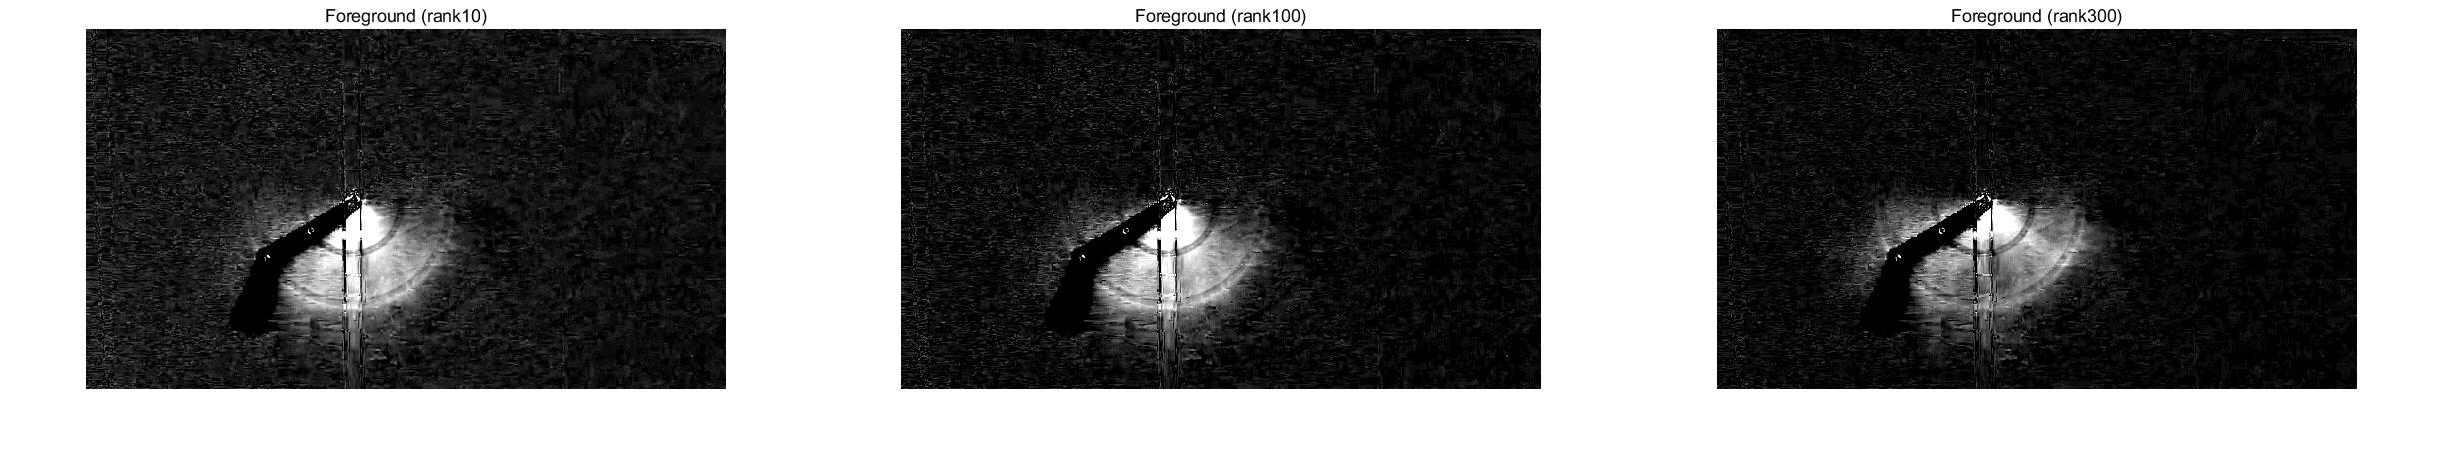
\includegraphics[scale=0.17]{t1f2.jpg}
\caption{Foreground video/Sparse reconstruction of varying rank (Test 1)}
\end{center}
\end{figure}
Verified by figure 3, increasing the rank of reconstruction did not create huge difference in terms of resolution.

\begin{figure}[H]
\begin{center}
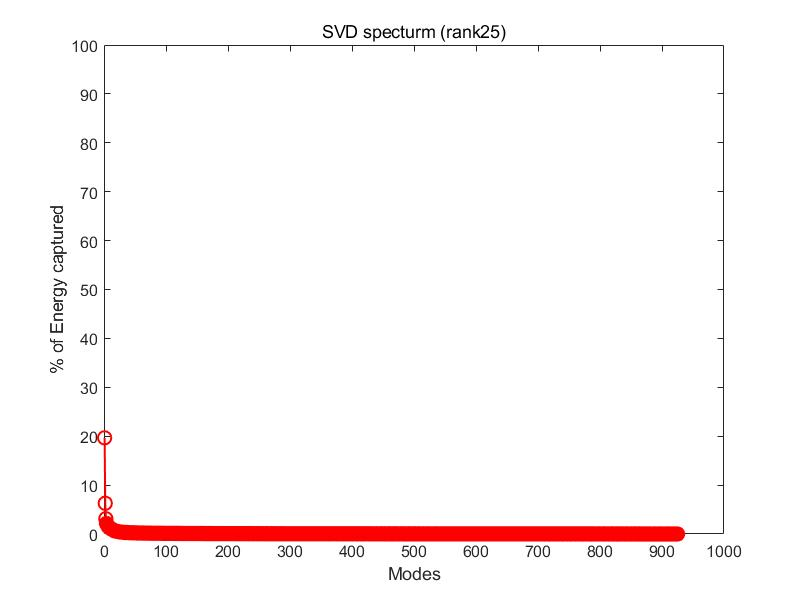
\includegraphics[scale=0.25]{t2f0.jpg}
\caption{SVD spectrum of energy captured by each mode (Test 2)}
\end{center}
\end{figure}
Similar test performed as showed in figure 4, but we notice that this time, the energy captured by first few modes dropped down significantly. Which is reasonable because human generally perform more complex movements.
\begin{figure}[H]
\begin{center}
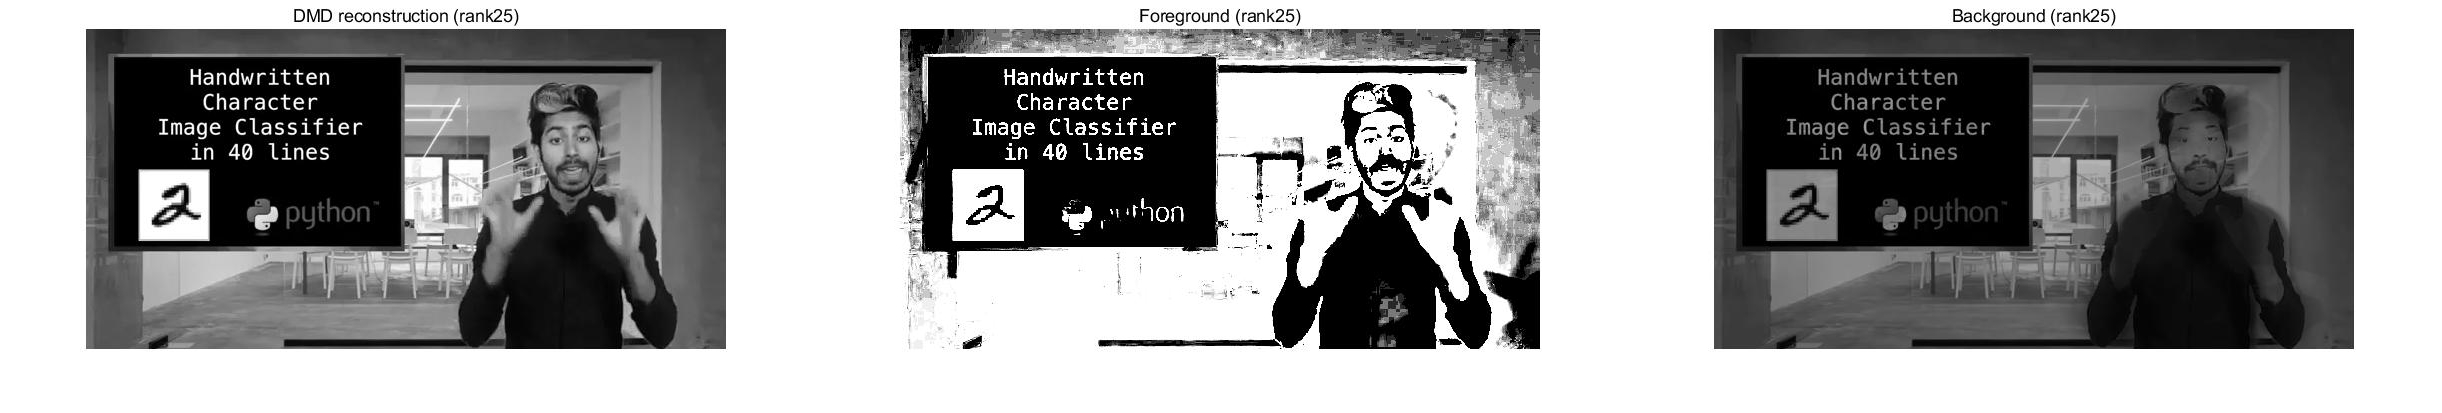
\includegraphics[scale=0.17]{t2f1.jpg}
\caption{DMD reconstruction (left), Foreground video/Sparse reconstruction(mid) and Background video/Low-rank reconstruction(right) of rank 25 (Test 2)}
\end{center}
\end{figure}

\begin{figure}[H]
\begin{center}
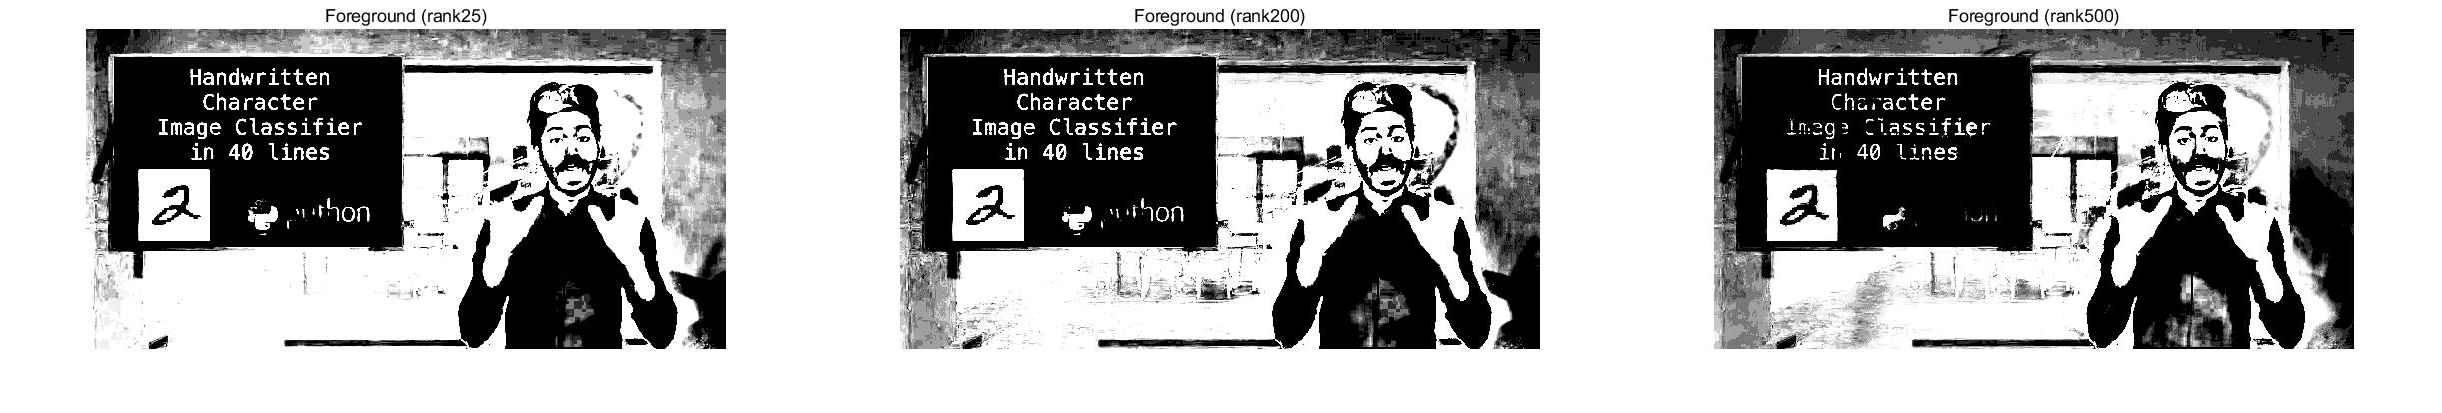
\includegraphics[scale=0.17]{t2f2.jpg}
\caption{Foreground video/Sparse reconstruction of varying rank (Test 2)}
\end{center}
\end{figure}

\begin{figure}[H]
\begin{center}
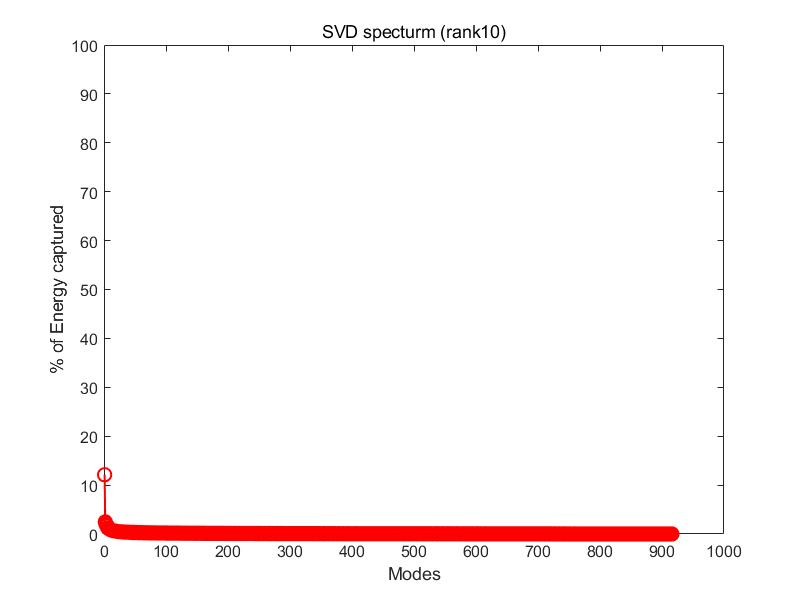
\includegraphics[scale=0.25]{t3f0.jpg}
\caption{SVD spectrum of energy captured by each mode (Test 3)}
\end{center}
\end{figure}
Energy captured by first few modes dropped even more in test 3. This may due to the non-stationary camera.

\begin{figure}[H]
\begin{center}
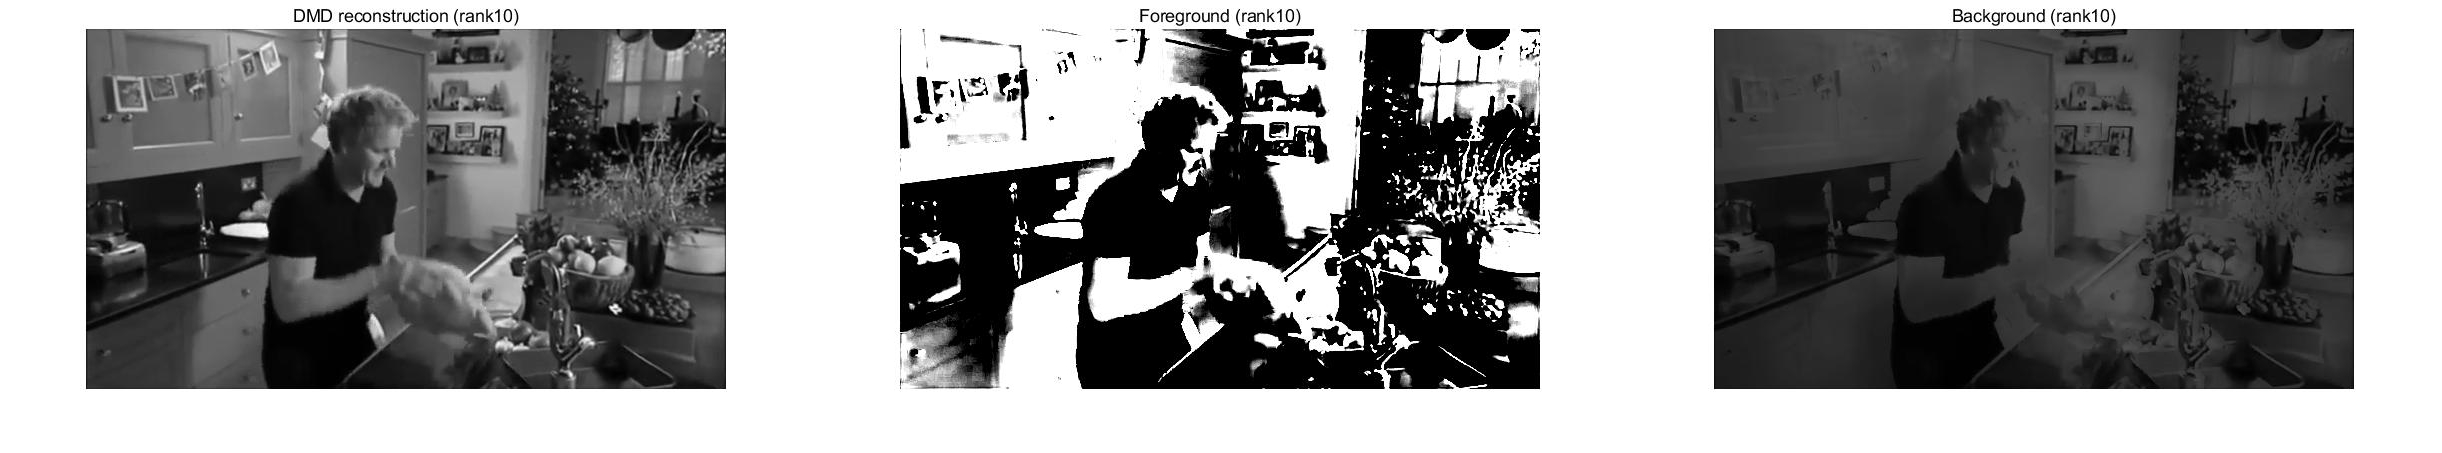
\includegraphics[scale=0.17]{t3f1.jpg}
\caption{DMD reconstruction (left), Foreground video/Sparse reconstruction(mid) and Background video/Low-rank reconstruction(right) of rank 10 (Test 3)}
\end{center}
\end{figure}

\begin{figure}[H]
\begin{center}
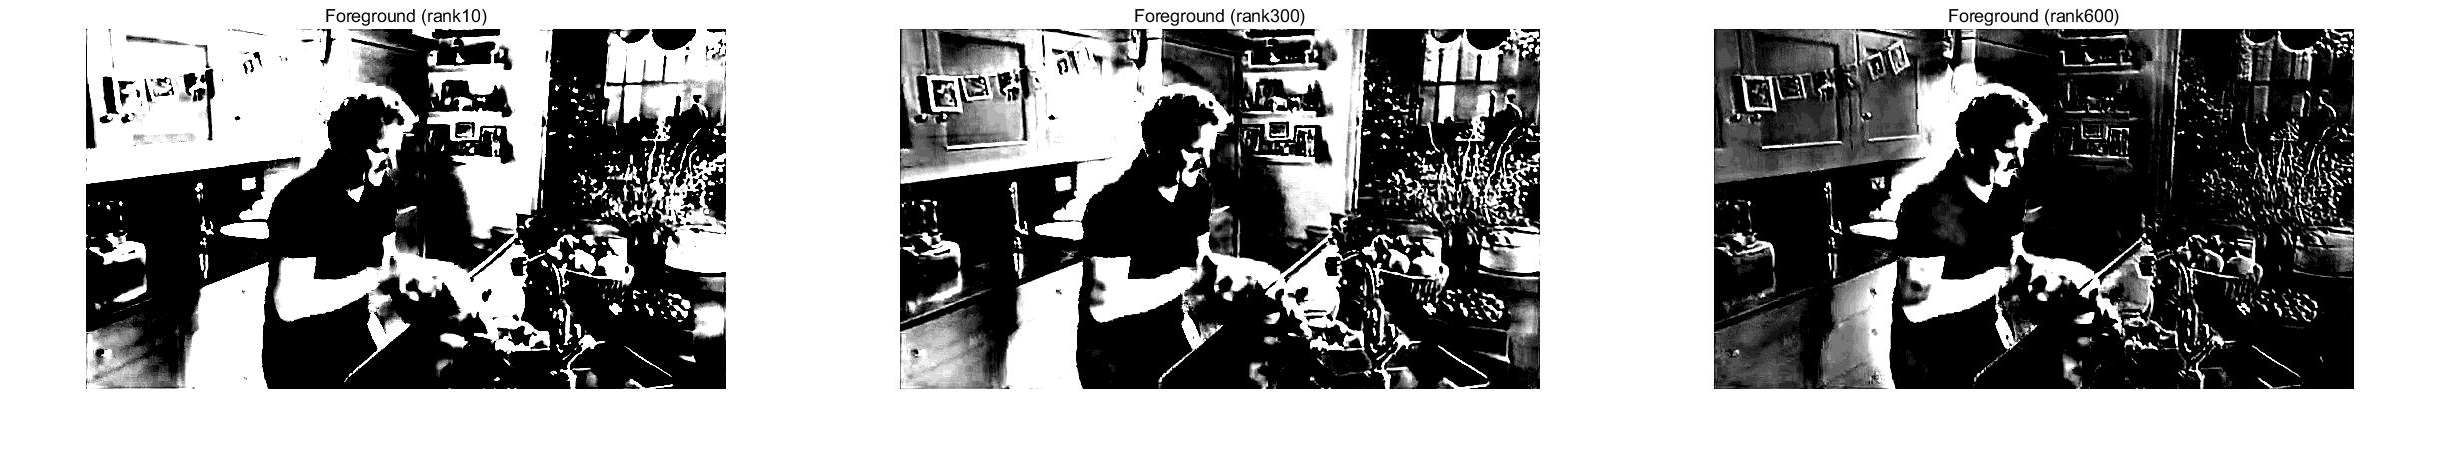
\includegraphics[scale=0.17]{t3f2.jpg}
\caption{Foreground video/Sparse reconstruction of varying rank (Test 3)}
\end{center}
\end{figure}
Verified by figure 9, we see that motion of surrounding objects were also extracted as foreground objects due to the motion of camera. We will need a much higher rank to fully extract interested foreground video, which takes significantly more time.

\section{Summary and Conclusions}
The above three tests have shown that DMD has comparatively good performance in separating foreground and background objects. However, by comparing test 2 and 3, we see that even for similar movements performed by human, non-stationary camera critically challenges the efficiency of DMD method so that low-rank reconstruction accuracy drops down significantly. This implies that DMD is only suitable for stationary backgrounds.


\begin{thebibliography}{11}
	\bibitem{dmd1}
	Kutz et al. 2016.
	\textit{Dynamic Mode Decomposition: Data-Driven Modeling of Complex Systems}. p. 2-19 https://doi.org/10.1137/1.9781611974508
	
	\bibitem{mtlb}
	\textit{Matlab Documentation. Mathworks}; [2019 Feb 25]. \\https://www.mathworks.com/help/index.html

	\bibitem{fore}
	\textit{Foreground detection. Wikipedia}; [2019 Mar 15]. \\https://www.en.wikipedia.org/wiki/Foreground\_Detection

	\bibitem{dmd2}
	\textit{Dynamic mode decomposition. Wikipedia}; [2019 Feb 25]. \\https://www.en.wikipedia.org/wiki/Dynamic\_Mode\_Decomposition
\end{thebibliography}


\section*{Appendix A: MATLAB functions used}
	\begin{itemize}
		\item \texttt{strcat}\\
		Concatenate strings horizontally
		\item \texttt{VideoReader}\\
		Creates object v to read video data from the file named filename
		\item \texttt{rgb2gray}\\
		Convert RGB image or colormap to grayscale
		\item \texttt{readFrame}\\
		Read video frame from video file
		\item \texttt{eig}\\
		"[V,D] = eig(A)" returns diagonal matrix "D" of eigenvalues and matrix "V "whose columns are the corresponding right eigenvectors.
		\item \texttt{svd}\\
		\texttt{[U,S,V] = svd(A)} performs a singular value decomposition of matrix \texttt{A}, such that \texttt{A = U*S*V'}
		
		\item \texttt{diag}\\
		\texttt{x = diag(A)} returns a column vector of the main diagonal elements of A.

	\end{itemize}


\section*{Appendix B: MATLAB codes}
\lstinputlisting{h5.m}




\end{document}
